% LaTeX template for Artifact Evaluation V20170622
%
% Prepared by Grigori Fursin (cTuning foundation, France and dividiti, UK),
% Bruce Childers (University of Pittsburgh, USA),
% Thierry Moreau (University of Washington, USA)
%
% See example of this Artifact Appendix in the CGO'17 paper (with the CK workflow framework):
% https://www.cl.cam.ac.uk/~sa614/papers/Software-Prefetching-CGO2017.pdf
%
% (C)opyright 2014-2017
%
% CC BY 4.0 license
%

\documentclass[sigplan]{acmart}

\usepackage{booktabs} % For formal tables

\usepackage{caption}
\usepackage{graphicx}
\usepackage{multirow}
\usepackage{nicefrac}
\usepackage{booktabs}
\usepackage{colortbl}
\usepackage{xcolor}
%\usepackage[hyphens]{url}
\usepackage{url}
\usepackage{romannum}
\usepackage{listings}
\usepackage{flushend}

\definecolor{dkgreen}{rgb}{0,0.6,0}
\definecolor{gray}{rgb}{0.5,0.5,0.5}
\definecolor{mauve}{rgb}{0.58,0,0.82}

\newcommand*{\x}{\mathsf{x}\mskip1mu}

\newenvironment{packed_itemize}{
\begin{itemize}
  \setlength{\itemsep}{1pt}
  \setlength{\parskip}{0pt}
  \setlength{\parsep}{0pt}
}{\end{itemize}}


% Copyright
%\setcopyright{none}
%\setcopyright{acmcopyright}
%\setcopyright{acmlicensed}
%\setcopyright{rightsretained}
%\setcopyright{usgov}
%\setcopyright{usgovmixed}
%\setcopyright{cagov}
%\setcopyright{cagovmixed}


% DOI
\acmDOI{10.1145/3229762.3229765}

% ISBN
% \acmISBN{123-4567-24-567/08/06}

%Conference
\acmConference[ReQuEST at ASPLOS'18]{1st ACM Reproducible Quality-Efficient Systems Tournament on Co-designing Pareto-efficient Deep Learning}{March 2018}{Williamsburg, VA, USA}
\acmYear{2018}
\copyrightyear{2018}

%\acmPrice{15.00}

%\acmBadgeL[http://ctuning.org/ae/ppopp2016.html]{ae-logo}
%\acmBadgeR[http://ctuning.org/ae/ppopp2016.html]{ae-logo} 

%>>>>>>>>>>>>>>>>>>>>>>>>>>>>>>>>>>>>>>>>>>>>>>>>>>>>>>>
\begin{document}

\title{Real-Time Image Recognition Using Collaborative IoT Devices}

\author{Ramyad Hadidi}
\affiliation{\institution{Georgia Institute of Technology}}
\email{rhadidi@gatech.edu}

\author{Jiashen Cao}
\affiliation{\institution{Georgia Institute of Technology}}
\email{jcao62@gatech.edu}

\author{Matthew Woodward}
\affiliation{\institution{Georgia Institute of Technology}}
\email{mwoodward@gatech.edu}

\author{Michael S. Ryoo}
\affiliation{\institution{ }}
\email{mryoo@egovid.com}

\author{Hyesoon Kim}
\affiliation{\institution{Georgia Institute of Technology}}
\email{hyesoon@cc.gatech.edu}

\renewcommand{\shortauthors}{}
\renewcommand{\shorttitle}{}

\maketitle


%>>>>>>>>>>>>>>>>>>>>>>>>>>>>>>>>>>>>>>>>>>>>>>>>>>>>>>>
\begin{abstract}
%
Internet of things (IoT) devices capture and create various forms of sensor data such as images and videos. However, such resource-constrained devices lack the capability to efficiently process data in a timely and real-time manner. Therefore, IoT systems strongly rely on a powerful server (either local or on the cloud) to extract useful information from data. In addition, during communication with servers, unprocessed, sensitive, and private data is transmitted throughout the Internet, a serious vulnerability. What if we were able to harvest the aggregated computational power of already existing IoT devices in our system to locally process this data? In this artifact, we utilize Musical Chair~\cite{musical-chair}, which enables efficient, localized, and dynamic real-time recognition by harvesting the aggregated computational power of these resource-constrained IoT devices. We apply Musical chair to two well-known image recognition models, AlexNet and VGG16, and implement them on a network of Raspberry PIs (up to 11). We compare inference per second and energy per inference of our systems with Tegra TX2, an embedded low-power platform with a six-core CPU and a GPU. We demonstrate that the collaboration of IoT devices, enabled by Musical Chair, achieves similar real-time performance without the extra costs of maintaining a server. 
%
\end{abstract}
%\vspace{-30pt}
%>>>>>>>>>>>>>>>>>>>>>>>>>>>>>>>>>>>>>>>>>>>>>>>>>>>>>>>

\section{Extended Abstract}

Musical Chair~\cite{musical-chair} is a technique for distributing deep neural network (DNN) models over several devices. DNN models have a variety of layers such as fully connected \texttt{(fc)}, convolution \texttt{(conv)}, batch normalization \texttt{(norm)}, max pooling \texttt{(maxpool)}, and activation \texttt{(act)} layers. Among these layers, fully connected and convolution layers are one the most resource-hungry and compute-intensive. Therefore, Musical Chair~\cite{musical-chair} aims at alleviating the compute cost and overcome the resource barrier of these layers by distributing their computation. In the paper, we discuss two modes of distributing these layers: data parallelism and model parallelism. Model parallelism is splitting parts of a given layer or group of layers over multiple devices, whereas data parallelism is providing the next input to multiple devices in a network. Note that we are examining this problem in the context of real-time data processing, in which we have a continuous stream of input data. In summary, for \texttt{conv} layers, data parallelism yields a higher performance in comparison with model parallelism. On the other hand, for \texttt{fc} layers, depending on the size of the input and the \texttt{fc} layer, the choice between model- and data-parallelism varies. As discussed in the paper, this is because of the resource-constrained nature of IoT devices. In this section, first, we explain our devices, then, describe Alexnet~\cite{kri:sut12} and VGG16~\cite{sim:zis14-deep} models, and finally, present Musical Chair task assignments for these models.


%>>>>>>>>>>>>>>>>>>>>>>>>>>>>>>>>>>>>>>>>>>>>>>>>>>>>>>>
\subsection{Technical Description}
%
%
%
\noindent {\bf Hardware/Software Overview}: 
In our implementation of a distributed IoT network, we use several Raspberry PIs~\cite{pi3}, the specification of which is shown in Table~\ref{tab:pi}. We choose Raspberry PI since it is a cheap and accessible platform that represents low-end IoT devices. On each PI, with the Ubuntu 16.04 operating system, we use Keras 2.1~\cite{chollet2015keras} with the TensorFlow 1.5~\cite{tensorflow2015-whitepaper} backend. Some arbitrary Raspberry PIs are equipped with a camera~\cite{pi3-cam} as well for demo purposes. But, for measurement purposes, these cameras are not required since inputs can be populated with random numbers instead of images. For power measurements, using a power analyzer, we measured the consumed power of a powered USB 3.0 hub that powers all Raspberry PIs. Moreover, timing measurements are done in the source code. To compare our collaborative IoT implementations, we also measure the performance and power consumption of our models on Jetson TX2~\cite{jetson}. the specification of which is in Table~\ref{tab:jetson}.


\renewcommand{\arraystretch}{0.7}
\begin{table}[t]
    \small
	\centering
	\vspace{-10pt}
	\captionsetup{singlelinecheck=on,aboveskip=1pt}
	\caption{Raspberry PI 3 specification~\cite{pi3}}
	\begin{tabular}{c | c | c}
		\toprule
        CPU & \multicolumn{2}{c}{1.2\,GHz Quad Core ARM Cortex-A53} \\
        Memory &  \multicolumn{2}{c}{900\,MHz 1\,GB RAM LPDDR2} \\
        GPU & \multicolumn{2}{c}{No GPGPU Capability} \\
        Price & \multicolumn{2}{c}{\$35 (Board) + \$5 (SD Card)} \\
        \midrule
        \multirow{3}{2cm}{\centering Power Consumption }
        &Idle (No Power Gating) & 1.3\,W \\
        &\%100 Utilization & 6.5\,W \\
        & Averaged Observed & 3\,W \\
		\bottomrule
	\end{tabular}
	\label{tab:pi}
	\vspace{-10pt}
\end{table} \renewcommand{\arraystretch}{1}


\renewcommand{\arraystretch}{0.7}
\begin{table}[t]
    \small
	\centering
	\vspace{0pt}
	\captionsetup{singlelinecheck=on,aboveskip=1pt}
	\caption{Nvidia Jetson TX2 specifications~\cite{jetson}.}
	\begin{tabular}{c | c | c}
		\toprule
        \multirow{2}{*}{\centering CPU } & \multicolumn{2}{c}{2.00\,GHz Dual Denver 2 +} \\
        & \multicolumn{2}{c}{2.00\,GHz Quad Core ARM Cortex-A57} \\
        \arrayrulecolor{black!20}\midrule\arrayrulecolor{black}
        Memory &  \multicolumn{2}{c}{1600\,MHz 8\,GB RAM LPDDR4} \\
        GPU & \multicolumn{2}{c}{Pascal Architecture - 256 CUDA Core} \\
        Total Price & \multicolumn{2}{c}{\$600} \\
        \midrule
        \multirow{3}{2cm}{\centering Power Consumption }
        &Idle (Power Gated)  & 5\,W \\
        &\%100 Utilization & 15\,W \\
        &Averaged Observed & 9.5\,W \\
		\bottomrule
	\end{tabular}
	\label{tab:jetson}
	\vspace{-10pt}
\end{table} \renewcommand{\arraystretch}{1}



%
%
%
%>>>>>>>>>>>>>>>>>>>>>>>>>>>>>>>>>>>>>>>>>>>>>>>>>>>>>>>
\noindent {\bf Models Overview}: We study single-stream Alexnet and VGG16 image recognition models, the architecture of which is shown in Figures~\ref{fig:alexnet} and \ref{fig:vgg16}, respectively.
%
%
\begin{figure}[h]
\centering
\vspace{-5pt}
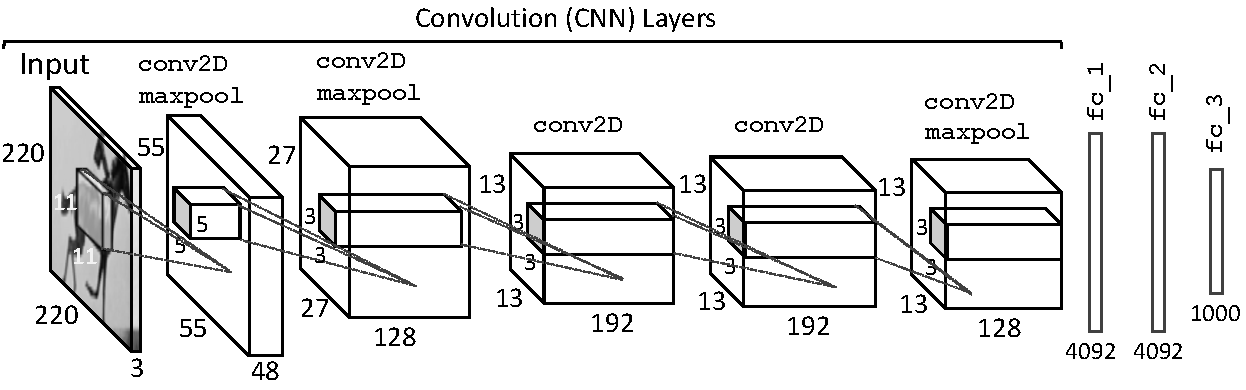
\includegraphics[width=1.0\linewidth]{figures/alexnet.pdf}
\captionsetup{singlelinecheck=on,aboveskip=3pt, belowskip=0pt}
\caption{Single stream AlexNet model.}
\label{fig:alexnet}
\vspace{-8pt}
\end{figure}
%
%
\begin{figure}[h]
\centering
\vspace{-5pt}
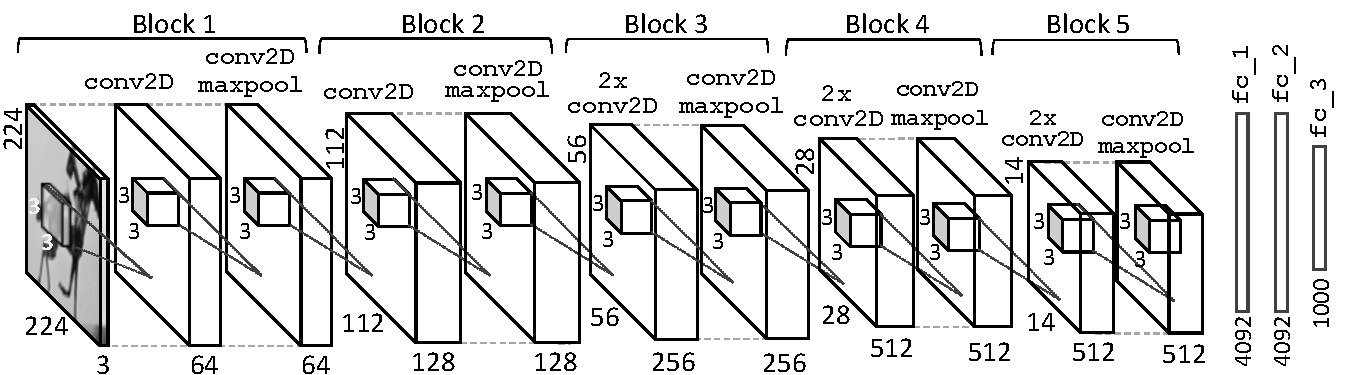
\includegraphics[width=1.0\linewidth]{figures/vgg16.pdf}
\captionsetup{singlelinecheck=on,aboveskip=5pt, belowskip=0pt}
\caption{VGG16 model.}
\label{fig:vgg16}
\vspace{-8pt}
\end{figure}
%
%
%

%>>>>>>>>>>>>>>>>>>>>>>>>>>>>>>>>>>>>>>>>>>>>>>>>>>>>>>>
\noindent {\bf Distributed Models}: After applying Musical Chair, for Alexnet, Figure~\ref{fig:alexnet-system} illustrates generated system architectures for five- and six-devices. In the five-device system, model parallelism is applied on the \texttt{fc\_1} layer, whereas, in six-device configuration, an additional data parallelism is performed on \texttt{conv} layers. For VGG16, Figure~\ref{fig:vgg16-system} depicts two generated systems for nine and 11 devices. In both systems, \texttt{fc\_1} is divided since its input size is extremely large, while, since the computation of \texttt{fc\_2} and \texttt{fc\_3} are not a bottleneck, Musical Chair prioritize the distribution of other layers such as \texttt{conv} layers using data parallelism.

%
%
\begin{figure}[h]
\centering
\vspace{-10pt}
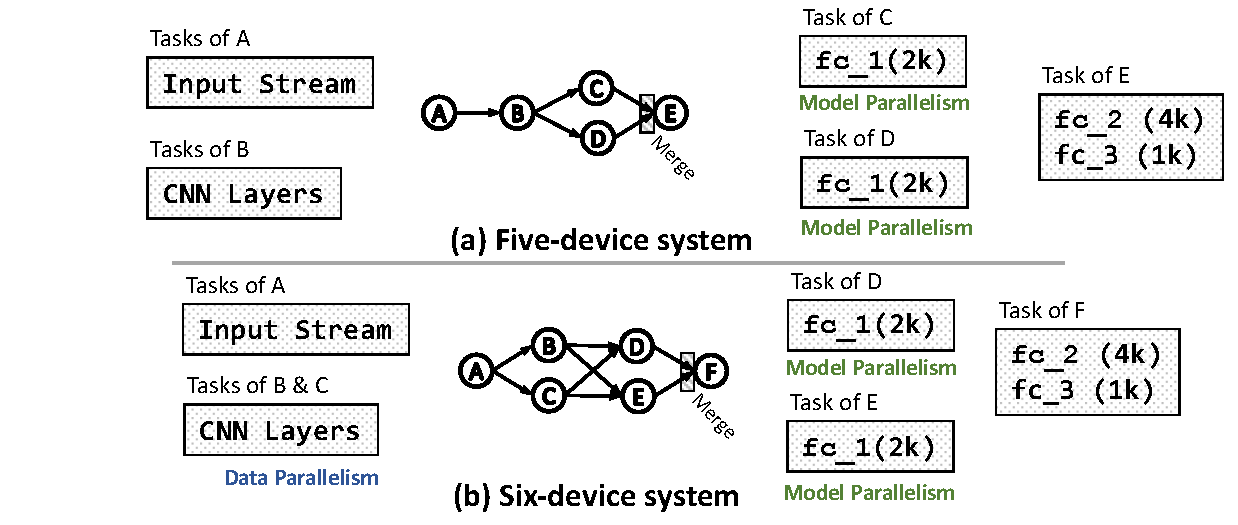
\includegraphics[width=1.0\linewidth]{figures/alexnet-nodes.pdf}
\captionsetup{singlelinecheck=on,aboveskip=0pt, belowskip=0pt}
\caption{System architectures for AlexNet.}
\label{fig:alexnet-system}
\vspace{-10pt}
\end{figure}
%
%
\begin{figure}[h]
\centering
\vspace{-5pt}
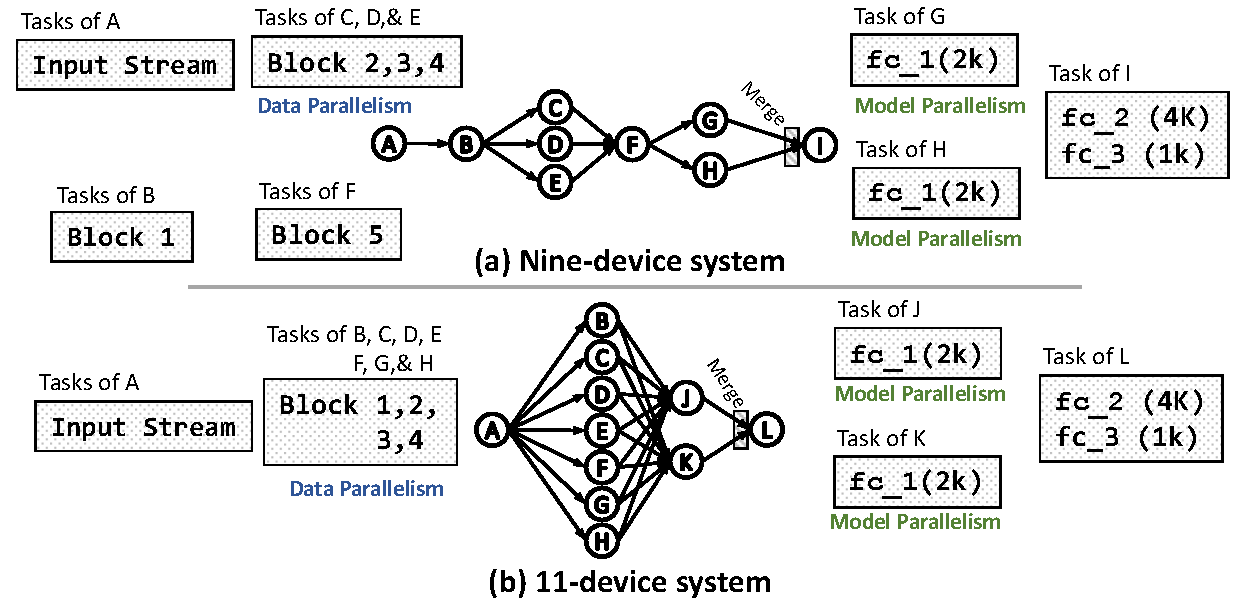
\includegraphics[width=1.0\linewidth]{figures/vgg-8nodes.pdf}
\captionsetup{singlelinecheck=on,aboveskip=5pt, belowskip=0pt}
\caption{System architectures for VGG16.}
\label{fig:vgg16-system}
\vspace{-15pt}
\end{figure}
%
%


%>>>>>>>>>>>>>>>>>>>>>>>>>>>>>>>>>>>>>>>>>>>>>>>>>>>>>>>
\subsection{Empirical Evaluation}
%
%
Figure~\ref{fig:alexnet-res}a depicts performance in terms of inference per second (IPS) for Alexnet. The performance of six-device system is similar to TX2 with CPU, while its performance is only 30\% worst than TX2 with GPU. Figure~\ref{fig:alexnet-res}b and c shows power consumption of all systems. As shown, the static energy consumption of the systems with Raspberry PIs are significantly higher, this is because (\romannum{1}) Raspberry PIs have several several unnecessary peripherals enabled, (\romannum{2}) TX2 is a low-power design with power gating capability, and (\romannum{3}) Raspberry PIs utilize more number of communication modules. Even so, we observe that systems with Raspberry PIs achieve better dynamic energy consumption. Figure~\ref{fig:vgg16-res} illustrates similar metrics for VGG16 model. Since VGG16 is more computationally intensive, we use more devices in our systems to achieve similar performance with TX2. When the number of devices increases from nine to 11, we achieve 2.3$\x$ better performance by reassigning all CNN blocks and performing more optimal data parallelism. In fact, compared to the TX2 with GPU, the 11-device system achieves comparable IPS (15\% degradation).


%
%
\begin{figure}[h]
\centering
\vspace{-5pt}
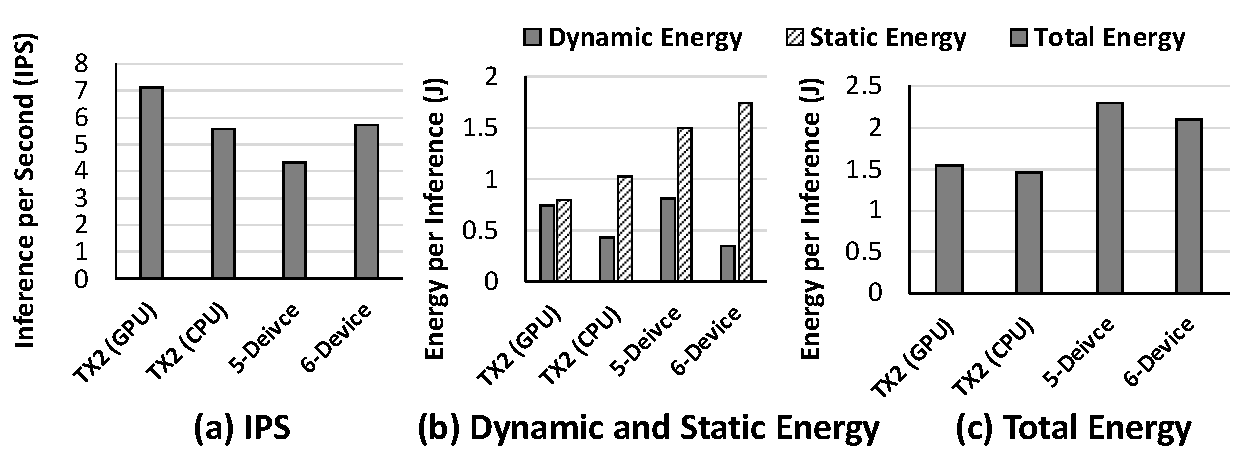
\includegraphics[width=1.0\linewidth]{figures/alexnet-res.pdf}
\captionsetup{singlelinecheck=on,aboveskip=5pt, belowskip=0pt}
\caption{AlexNet: Measured IPS (a), static and dynamic energy consumption (b), and total energy consumption (c).}
\label{fig:alexnet-res}
\vspace{-15pt}
\end{figure}
%
%
\begin{figure}[h]
\centering
\vspace{0pt}
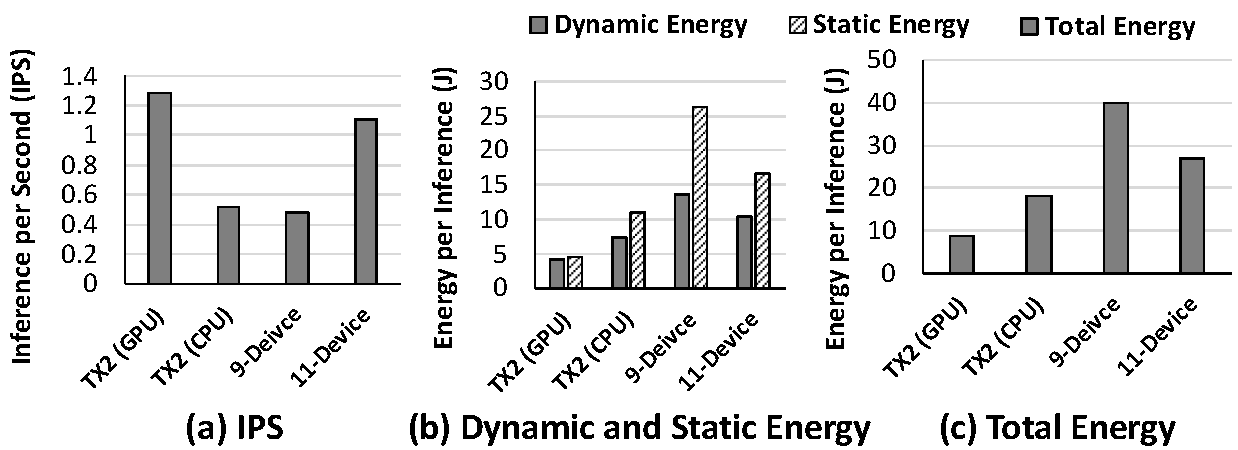
\includegraphics[width=1.0\linewidth]{figures/vgg16-res.pdf}
\captionsetup{singlelinecheck=on,aboveskip=5pt, belowskip=0pt}
\caption{VGG16: Measured IPS (a), static and dynamic energy consumption (b), and total energy consumption (c).}
\label{fig:vgg16-res}
\vspace{-10pt}
\end{figure}
%
%



%%%%%%%%%%%%%%%%%%%%%%%%%%%%%%%%%%%%%%%%%%%%%%%%%%%%
\bibliographystyle{ACM-Reference-Format}

\begin{thebibliography}{}
%\softraggedright

\bibitem{kri:sut12}
A.~Krizhevsky, I.~Sutskever, and G.~E. Hinton, ``{Imagenet Classification With
  Deep Convolutional Neural Networks},'' in {\em Advances in Neural Information
  Processing Systems (NIPS)}, pp.~1097--1105, 2012.
  
\bibitem{sim:zis14-deep}
K.~Simonyan and A.~Zisserman, ``{Very Deep Convolutional Networks for
  Large-Scale Image Recognition},'' in {\em International Conference on
  Learning Representations (ICLR)}, 2015.
  
\bibitem{musical-chair}
R.~{Hadidi}, J.~{Cao}, M.~{Woodward}, M.~{Ryoo}, and H.~{Kim}, ``{Musical
  Chair: Efficient Real-Time Recognition Using Collaborative IoT Devices},''
  {\em ArXiv e-prints:1802.02138}.
  
\bibitem{rus:den15}
O.~Russakovsky, J.~Deng, H.~Su, J.~Krause, S.~Satheesh, S.~Ma, Z.~Huang,
  A.~Karpathy, A.~Khosla, M.~Bernstein, {\em et~al.}, ``{Imagenet Large Scale
  Visual Recognition Challenge},'' {\em International Journal of Computer
  Vision (IJCV)}, vol.~115, no.~3, pp.~211--252, 2015.
  
\bibitem{pi3}
R.~P. Foundation, ``{Raspberry Pi 3}.''
  \url{https://www.raspberrypi.org/products/raspberry-pi-3-model-b/}, 2018.
\newblock [Online; accessed 5/1/18].

\bibitem{jetson}
NVIDIA, ``{NVIDIA Jetson TX}.''
  \url{http://www.nvidia.com/object/embedded-systems-dev-kits-modules.html},
  2017.
\newblock [Online; accessed 5/1/18].

\bibitem{chollet2015keras}
F.~Chollet {\em et~al.}, ``{Keras}.'' \url{https://github.com/fchollet/keras},
  2015.
  
\bibitem{tensorflow2015-whitepaper}
M.~Abadi {\em et~al.}, ``{{TensorFlow}: Large-Scale Machine Learning on
  Heterogeneous Systems},'' 2015.
\newblock Software available from tensorflow.org.

\bibitem{pi3-cam}
R.~P. Foundation, ``{Raspberry Pi 3}.''
  \url{https://www.raspberrypi.org/products/camera-module-v2/}, 2018.
\newblock [Online; accessed 5/1/18].

\bibitem{apache}
T.~A.~S. Foundation, ``{Apache Avro}.'' \url{https://avro.apache.org}, 2018.
\newblock [Online; accessed 5/1/18].

\bibitem{jetpack}
NVIDIA, ``{NVIDIA JetPack}.'' \url{https://developer.nvidia.com/embedded/jetpack}, 2018.
\newblock [Online; accessed 5/1/18].

\bibitem{request-asplos18}
{ReQuEST at ASPLOS'18:}, ``1st Reproducible Tournament on Pareto-efficient Image Classification.''
    \url{http://cknowledge.org/request-cfp-asplos2018.html},
    2018.
\newblock [Online; accessed 5/1/18].

\bibitem{cm:29db2248aba45e59:0c7348dfbadd5b95}
 Thierry Moreau, Anton Lokhmotov, Grigori Fursin, ``Introducing ReQuEST: an Open Platform for Reproducible and Quality-Efficient Systems-ML Tournaments,''
  {\em arXiv 1801.06378}, 2018.

\end{thebibliography}
%%%%%%%%%%%%%%%%%%%%%%%%%%%%%%%%%%%%%%%%%%%%%%%%%%%%

%>>>>>>>>>>>>>>>>>>>>>>>>>>>>>>>>>>
\newpage

\onecolumn

\appendix
\section{Artifact Appendix}

Submission and reviewing methodology: \\
{\em http://cTuning.org/ae/submission-20171101.html}

%%%%%%%%%%%%%%%%%%%%%%%%%%%%%%%%%%%%%%%%%%%%%%%%%%%%%%%%%%%%%%%%%%%%%
\subsection{Abstract}

This Artifact Appendix describes experimental workflow,
artifacts and results from this paper evaluated 
during the 1st reproducible ReQuEST tournament at the ACM ASPLOS'18:

\begin{packed_itemize}
  \item {\bf Original artifact:} \url{https://github.com/parallel-ml/asplos2018-workshop}
  \item {\bf Latest CK workflow:} \url{https://github.com/ctuning/ck-request-asplos18-iot-farm}
  \item {\bf CK results:} \url{https://github.com/ctuning/ck-request-asplos18-results-iot-farm}
  \item {\bf Artifact DOI:} \url{https://doi.org/10.1145/3229771}
  \item {\bf ReQuEST submission and reviewing guidelines:} \url{http://cknowledge.org/request-cfp-asplos2018.html} (\cite{request-asplos18})
  \item {\bf ReQuEST goals:} \cite{cm:29db2248aba45e59:0c7348dfbadd5b95}
  \item {\bf ReQuEST workflows:} \url{https://github.com/ctuning/ck-request-asplos18-results}
  \item {\bf ReQuEST scoreboard:} \url{http://cKnowledge.org/request-results}
\end{packed_itemize}

Our artifact provides source code for all of our
implementations on a public Github repository. The source
codes allows the evaluation of our results on a network
of connected Raspberry PI 3s and Nvidia Jetson TX2. Note that
for measuring the energy consumption, a power analyzer
is needed. Additionally, to measure the energy consumption
of several Raspberry PIs, we utilize a powered USB 3.0 hub and
measure its energy consumption with the power analyzer.

%%%%%%%%%%%%%%%%%%%%%%%%%%%%%%%%%%%%%%%%%%%%%%%%%%%%%%%%%%%%%%%%%%%%%
\subsection{Artifact check-list}

Details: \url{http://cTuning.org/ae/submission_extra.html}

\begin{itemize}
  \item {\bf Algorithm:} Image recognition models of Alexnet and VGG16.
  \item {\bf Program:} Written scripts in Keras framework.
  \item {\bf Compilation:} Python $\geq$ 2.7.
  %\item {\bf Transformations: }
  \item {\bf Binary:} will be compiled on a target platform.
  \item {\bf Data set:} Randomly generated images with Numpy (thus will not be able to test accuracy).
  \item {\bf Run-time environment:} Ubuntu 16.04 ; Python version $\geq$ 2.7; Keras $\geq$ 2.1.3 with Tensorflow-gpu $\geq$ 1.5 for the backend; \emph{(for Raspberry PI systems)} Apache Avro~\cite{apache} $\geq$ 1.8.2; \emph{(for TX2 GPU)} CUDA 8.0 with cuDNN $\geq$ 5.1.
  \item {\bf Hardware:} Nvidia Jetson TX2 ; up to 11 Raspberry PI 3 with 16\,GB SD cards; power analyzer; Wifi router (we use 300Mbps, 2.4\,GHz 802.11n).
  %\item {\bf Run-time state: }
  \item {\bf Execution:} Automated via CK command line
  \item {\bf Metrics:} Inference per second; static and dynamic energy consumption.
  \item {\bf Output:} Scripts output end-to-end latency. User measures power consumption during idle state and inference operations.
  \item {\bf Experiments:} Performing inference on different hardware.
  \item {\bf How much disk space required (approximately)?}
  \item {\bf How much time is needed to prepare workflow (approximately)?}
  \item {\bf How much time is needed to complete experiments (approximately)?}
  \item {\bf Publicly available?:} Yes
  \item {\bf Code license(s)?:} 
  \item {\bf CK workflow framework used?} Yes
  \item {\bf CK workflow URL:} \url{https://github.com/ctuning/ck-request-asplos18-iot-farm}
  \item {\bf CK results URL:} \url{https://github.com/ctuning/ck-request-asplos18-results-iot-farm}
  \item {\bf Original artifact:} \url{https://github.com/parallel-ml/asplos2018-workshop}

\end{itemize}

%%%%%%%%%%%%%%%%%%%%%%%%%%%%%%%%%%%%%%%%%%%%%%%%%%%%%%%%%%%%%%%%%%%%%
\subsection{Description}
%
%
\subsubsection{How delivered}
Our source code and scripts are available on Github: \url{https://github.com/parallel-ml/asplos2018-workshop}.
A brief guide, similar to this artifact, is also available at \texttt{README.md} in the repository.

%
%
\subsubsection{Hardware dependencies}
We use Nvidia Jetson TX2 for the first part of the experiments. In the second part, we utilize up to 11 Raspberry PI 3s. In addition, a wifi router is necessary for the connection between Raspberry PIs. For both part, a conventional power analyzer is needed to measure the power consumption of its output. To easily measure the power consumption of Raspberry PIs, the usage of a powered USB 3.0 hub is recommended.

%
%
\subsubsection{Software dependencies}
Both our hardware, TX2 and Raspberry PI, are AArch64 architectures. We use Ubuntu 16.04 on both systems, however, similar Linux distribution should also work. On TX2, we use NVIDIA JetPack 3.0 to install CUDA 8.0 and cuDNN 5.1. Then, we utilize \texttt{pip}, a Python package manager, to install Keras with a Tensorflow-gpu backend, this installation procedure is similar on Raspberry PI as well. In addition, for Raspberry PI, we install Apache Avro through \texttt{pip} for managing remote procedure calls (RPC). 


%\subsubsection{Data sets}

%%%%%%%%%%%%%%%%%%%%%%%%%%%%%%%%%%%%%%%%%%%%%%%%%%%%%%%%%%%%%%%%%%%%%
\subsection{Installation}

\noindent {\bf TX2:} After installing a Linux distribution on TX2 (we use Ubuntu 16.04), install Nvidia JetPack~\cite{jetpack} for enabling GPU support (CUDA and cuDNN). After installing Python and \texttt{pip}, install Keras through \texttt{pip}. Keras should be able to install its dependencies with \texttt{pip} automatically. If not, follow the Keras guide, the url of which is in the \texttt{README.md}.

\noindent {\bf Raspberry PI:} For connivence of not repeating every step on all 11 Raspberry PIs, we suggest that performing all steps on a single Raspberry PI and then cloning its SD card. We have provided dependency file in the repo for CPU-based installation. You can execute it with bellow command to install packages:
\begin{lstlisting}
  pip install -r requirements.txt
\end{lstlisting}

\noindent Moreover, make sure ports number 12345 and 9999 are open on all Raspberry PIs and your router. Then, get all of the IP addresses of Raspberry PIs in your network, and fill them in \texttt{resource/ip} files under \texttt{mutiple-devices/\{experiment\}} dir based on Figures~\ref{fig:alexnet-system} and \ref{fig:vgg16-system}. The files are in the JSON format and each task is assigned with a list of IPs. For instance, for VGG16, in nine-device system (Figure~\ref{fig:vgg16-system}a), you should have three devices for \texttt{block234} and two devices for \texttt{fc\_1}.


%%%%%%%%%%%%%%%%%%%%%%%%%%%%%%%%%%%%%%%%%%%%%%%%%%%%%%%%%%%%%%%%%%%%%
\subsection{Experiment workflow}

\noindent {\bf TX2:} Go to the \texttt{single-device} directory, the \texttt{predict.py} script in each model executes 50 inferences. Then, it reports the average time per inference. For energy measurements, first, measure the idle power of TX2 (static power), then, during inference time measure the consumed power (static and dynamic power). Use the commands below to execute CPU and GPU versions:
\begin{lstlisting}
  #GPU version
  python predict.py
  #CPU version
  CUDA_VISIBLE_DEVICE= python predict.py
\end{lstlisting}

\noindent {\bf Raspberry PI:}  Go to the \texttt{multiple-devices/\{experiment\}} directory on each Raspberry PI. On all of devices except the initial sender, execute:
\begin{lstlisting}
  python node.py
\end{lstlisting}
Then, start the data sender with:
\begin{lstlisting}
  python initial.py
\end{lstlisting}
The initial node receives the inference responses back from the end node and prints end-to-end latency and per-layer latency for each inference. For energy measurements, first, measure the idle power of the system (we use a 14-port powered USB 3.0 hub) (static power), then, during inference time measure the consumed power (static and dynamic power).

%%%%%%%%%%%%%%%%%%%%%%%%%%%%%%%%%%%%%%%%%%%%%%%%%%%%%%%%%%%%%%%%%%%%%
\subsection{Evaluation and expected result}

The expected results should be similar to Figures~\ref{fig:alexnet-res} and \ref{fig:vgg16-res}. In these figures, IPS, shown in subfigures a, is derived by dividing one by average end-to-end latency. Note that in Raspberry systems, since network congestion affects the latency, expect around 10\%--20\% variation in the results. For energy measurements, our power analyzer reports consumed power ($W/s$), so we multiply this reported number by end-to-end latency to derive total energy consumption per inference ($J$). To derive dynamic energy consumption, simply subtract static energy consumption (recorded during idle state) from total energy consumption (recorded during inference).


%%%%%%%%%%%%%%%%%%%%%%%%%%%%%%%%%%%%%%%%%%%%%%%%%%%%%%%%%%%%%%%%%%%%%
%\subsection{Experiment customization}

%%%%%%%%%%%%%%%%%%%%%%%%%%%%%%%%%%%%%%%%%%%%%%%%%%%%%%%%%%%%%%%%%%%%%
%\subsection{Notes}


\end{document}
